%%%%%%%%%%%%%%%%%%%%%%%%%%%%%%%%%%%%%%%%%%%%%%%%%%%%%%%%%%%%%
%% Begin exercise %%
%%%%%%%%%%%%%%%%%%%%%%%%%%%%%%%%%%%%%%%%%%%%%%%%%%%%%%%%%%%%%
\ex{Synchronous machines}


\normalsize{\textbf{Acknowledgement}: Parts of the following exercise are adapted from ``Elektrische Antriebstechnik'' by J. Böcker, Paderborn University, 2020
}\\



%%%%%%%%%%%%%%%%%%%%%%%%%%%%%%%%%%%%%%%%%%%%%%%%%%%%%%%%%%%%%
%% Task 1 %%
%%%%%%%%%%%%%%%%%%%%%%%%%%%%%%%%%%%%%%%%%%%%%%%%%%%%%%%%%%%%%

\task{Transient simulation of a salient pole synchronous machine}
Given is a salient pole synchronous machine with the parameters in Tab.~\ref{tab:para_salientSynchonousMachine}.

\begin{table}[htb]
    \caption{Parameters of the salient synchronous machine.}
    \centering
    \begin{tabular}{lll}\toprule
    Symbol  & Description       & Value \\
    \midrule
    $R_{\mathrm{s}}$    & Stator resistance         & $\SI{0.0196}{\Omega}$ \\
    $R_{\mathrm{f}}$    & Field winding resistance  & $\SI{54.7}{\Omega}$ \\
    $L_{\mathrm{s,d}}$    & Stator inductance d-axis  & $\SI{2.7}{\milli\henry}$ \\
    $L_{\mathrm{s,q}}$    & Stator inductance q-axis  & $\SI{1.3}{\milli\henry}$ \\
    $L_{\mathrm{f}}$    & Self field inductance     & $\SI{20.3}{\milli\henry}$ \\
    $M_{\mathrm{fs}}$   & Mutual inductance         & $\SI{92.8}{\milli\henry}$ \\
    $I_{\mathrm{n}}$    & Nominal stator current    & $\SI{450}{\ampere}$ \\
    $I_{\mathrm{f,n}}$  & Nominal field current     & $\SI{7.854}{\ampere}$ \\
    \bottomrule
    \end{tabular}
    \label{tab:para_salientSynchonousMachine}
\end{table}






%%%%%%%%%%%%%%%%%%%%%%%%%%%%%%%%%%%%%%%%%%%%%%%%%%%%%%%%%%%%%
\subtask{Calculate the transient response for $i_{\mathrm{dq}}$ and $i_{\mathrm{f}}$ if a short circuit occurs at the running machine. Assume $i_{\mathrm{d0}} = i_{\mathrm{q0}}$ = 0, $i_{\mathrm{f0}} = i_{\mathrm{f,n}}$ for $t=0$ and a fixed rotational speed $\omega_{\mathrm{r,el}}$. Assume further that the ohmic stator resistance can be neglected for the short-term transient response.}


\begin{solutionblock}
    
    The machine model is defined as
    \begin{align}
        \begin{split}
        \frac{\mathrm{d}}{\mathrm{d}t}
        &
        \begin{bmatrix}
            i_{\mathrm{s,d}}(t) \\
            i_{\mathrm{s,q}}(t) \\
            i_{\mathrm{f}}(t)
        \end{bmatrix}
        =
        \begin{bmatrix}
            -L_{\mathrm{f}}/\gamma  & 0 & M_{\mathrm{fs}}/\gamma \\
            0                       & 1/L_{\mathrm{s,q}}  & 0 \\
            M_{\mathrm{fs}}/\gamma  & 0 & -L_{\mathrm{s,d}}/\gamma 
        \end{bmatrix} \\
        &
        \begin{pmatrix}
            \begin{bmatrix}
                u_{\mathrm{s,d}}(t) \\
                u_{\mathrm{s,q}}(t) \\
                u_{\mathrm{f}}(t)
            \end{bmatrix}
            -
            \begin{bmatrix}
                R_{\mathrm{s}}  & 0 & 0 \\
                0 & R_{\mathrm{s}} & 0 \\
                0 & 0 & R_{\mathrm{f}}
            \end{bmatrix}
            \begin{bmatrix}
                i_{\mathrm{s,d}}(t) \\
                i_{\mathrm{s,q}}(t) \\
                i_{\mathrm{f}}(t)
            \end{bmatrix}
            -
            \begin{bmatrix}
                0 & -\omega_{\mathrm{r,el}}(t) & 0 \\
                \omega_{\mathrm{r,el}}(t) & 0 & 0 \\
                0 & 0 & 0
            \end{bmatrix}
            \begin{bmatrix}
                \psi_{\mathrm{s,d}}(t) \\
                \psi_{\mathrm{s,q}}(t) \\
                \psi_{\mathrm{f}}(t)
            \end{bmatrix}
        \end{pmatrix},
        \label{eq:model_sm}
    \end{split}
    \end{align}

    with the parameter 
    \begin{equation}
        \gamma = M_{\mathrm{fs}}^2-L_{\mathrm{s,d}}L_{\mathrm{f}},
    \end{equation}
    and the flux linkages
    \begin{equation}
        \begin{bmatrix}
            \psi_{\mathrm{s,d}}(t) \\
            \psi_{\mathrm{s,q}}(t) \\
            \psi_{\mathrm{f}}(t)
        \end{bmatrix}
        =
        \begin{bmatrix}
            L_{\mathrm{s,d}}  & 0     & M_{\mathrm{fs}} \\
            0       & L_{\mathrm{s,q}}    & 0 \\
            M_{\mathrm{fs}}     & 0     & L_{\mathrm{f}}
        \end{bmatrix}
        \begin{bmatrix}
            i_{\mathrm{s,d}}(t) \\
            i_{\mathrm{s,q}}(t) \\
            i_{\mathrm{f}}(t)
        \end{bmatrix}.
    \end{equation}



    With the assumption of a constant speed ($\omega_{\mathrm{r,el}}(t) =\omega_{\mathrm{r,el}}$), the general machine model from \eqref{eq:model_sm} is rewritten as follows:
    \begin{align}
        \begin{split}
        \frac{\mathrm{d}}{\mathrm{d}t}
        \begin{bmatrix}
            i_{\mathrm{s,d}}(t) \\
            i_{\mathrm{s,q}}(t) \\
            i_{\mathrm{f}}(t)
        \end{bmatrix}
        = &
        \begin{bmatrix}
            L_{\mathrm{f}}R_{\mathrm{s}}/\gamma     & -L_{\mathrm{f}}L_{\mathrm{s,q}}\omega_{\mathrm{r,el}}/\gamma & -M_{\mathrm{fs}}R_{\mathrm{f}}/\gamma \\
            -L_{\mathrm{s,d}}\omega_{\mathrm{r,el}}/L_{\mathrm{s,q}} & -R_{\mathrm{s}}/L_{\mathrm{s,q}} & -M_{\mathrm{fs}}\omega_{\mathrm{r,el}}/L_{\mathrm{s,q}} \\
            -M_{\mathrm{fs}}R_{\mathrm{s}}/\gamma & M_{\mathrm{fs}}L_{\mathrm{s,q}}\omega_{\mathrm{r,el}} / \gamma & L_{\mathrm{s,d}}R_{\mathrm{f}}/\gamma 
        \end{bmatrix}
        \begin{bmatrix}
            i_{\mathrm{s,d}}(t) \\
            i_{\mathrm{s,q}}(t) \\
            i_{\mathrm{f}}(t)
        \end{bmatrix}
        \\
        + &
        \begin{bmatrix}
            -L_{\mathrm{f}}/\gamma & 0 & M_{\mathrm{fs}}/\gamma \\
            0 & 1/L_{\mathrm{s,q}} & 0 \\
            M_{\mathrm{fs}}/\gamma & 0 & -L_{\mathrm{s,d}}/\gamma
        \end{bmatrix}
        \begin{bmatrix}
            u_{\mathrm{s,d}}(t) \\
            u_{\mathrm{s,q}}(t) \\
            u_{\mathrm{f}}(t)
        \end{bmatrix}.
    \end{split}
    \end{align}
    
    The exact system response is calculated with:
    \begin{equation}
        \bm{x}(t) = \bm{\Phi}(t,t_{\mathrm{0}})\bm{x}_{\mathrm{0}} + \int_{t_{\mathrm{0}}}^{t}\bm{\Phi}(t,\tau)\bm{B}\bm{u}(\tau) \mathrm{d}\tau,
    \end{equation}
    with
    \begin{equation}
        \bm{x}_{\mathrm{0}} = \bm{x}(t_{\mathrm{0}}),
    \end{equation}
    and,
    \begin{equation}
        \bm{\Phi}(t,t_{\mathrm{0}}) = e^{\bm{A}(t-t_{\mathrm{0}})}.
    \end{equation}
    

   To calculate the transient system response without damping, the resistances are assumed to be zero. Hence, the equation is simplifies to:
    \begin{align}
        \begin{split}
        \underbrace{
        \frac{\mathrm{d}}{\mathrm{d}t}
        \begin{bmatrix}
            i_{\mathrm{s,d}}(t) \\
            i_{\mathrm{s,q}}(t) \\
            i_{\mathrm{f}}(t)
        \end{bmatrix}}_{\frac{\mathrm{d}}{\mathrm{d}t}\bm{x}(t)}
        =
        &
        \underbrace{
        \begin{bmatrix}
            0   & -L_{\mathrm{f}}L_{\mathrm{s,q}}\omega_{\mathrm{r,el}}/ \gamma   & 0 \\
            -L_{\mathrm{s,d}}\omega_{\mathrm{r,el}}/ L_{\mathrm{s,q}} & 0 & -M_{\mathrm{fs}}\omega_{\mathrm{r,el}} / L_{\mathrm{s,q}} \\
            0 & M_{\mathrm{fs}}L_{\mathrm{s,q}}\omega_{\mathrm{r,el}} / \gamma & 0
        \end{bmatrix}}_{\bm{A}}
        \underbrace{
        \begin{bmatrix}
            i_{\mathrm{s,d}}(t) \\
            i_{\mathrm{s,q}}(t) \\
            i_{\mathrm{f}}(t)
        \end{bmatrix}}_{\bm{x}(t)}
        \\
        + &
        \underbrace{
        \begin{bmatrix}
            -L_{\mathrm{f}}/\gamma & 0 & M_{\mathrm{fs}}/\gamma \\
            0 & 1/L_{\mathrm{s,q}} & 0 \\
            M_{\mathrm{fs}}/\gamma & 0 & -L_{\mathrm{s,d}}/\gamma
        \end{bmatrix}}_{\bm{B}}
        \underbrace{
        \begin{bmatrix}
            u_{\mathrm{s,d}}(t) \\
            u_{\mathrm{s,q}}(t) \\
            u_{\mathrm{f}}(t)
        \end{bmatrix}}_{\bm{u}(t)}.
    \end{split}
    \end{align}

    The eigenvalues of $\bm{A}$ are determined by:
    \begin{align}
        \begin{split}
        &\mathrm{det}\left(
            \begin{bmatrix}
                \lambda & L_{\mathrm{f}}L_{\mathrm{s,q}}\omega_{\mathrm{r,el}} /\gamma & 0 \\
                L_{\mathrm{s,d}}\omega_{\mathrm{r,el}} / L_{\mathrm{s,q}} & \lambda & M_{\mathrm{fs}}\omega_{\mathrm{r,el}}/L_{\mathrm{s,q}} \\
                0 & -M_{\mathrm{fs}}L_{\mathrm{s,q}}\omega_{\mathrm{r,el}} / \gamma & \lambda
            \end{bmatrix}
        \right)
        = 0 \\
        &= \lambda^3 + \frac{M_{\mathrm{fs}}\omega_{\mathrm{r,el}}^2}{\gamma}\lambda - \frac{L_{\mathrm{f}}L_{\mathrm{s,d}}\omega_{\mathrm{r,el}}^2}{\lambda}\gamma \\
        &= \lambda\left(\lambda^2+\frac{\omega_{\mathrm{r,el}}^2}{\gamma}M_{\mathrm{fs}}^2-L_{\mathrm{f}}L_{\mathrm{s,d}}\right).
    \end{split}
    \end{align}

    This results in the following eigenvalues, $\lambda_{\mathrm{1,2,3}} = \left\{+\mathrm{j}\omega_{\mathrm{r,el}}, -\mathrm{j}\omega_{\mathrm{r,el}}, 0 \right\}$.


    The following transition matrix results from the calculated eigenvalues
    \begin{equation}
        \bm{\Phi}(t,t_{\mathrm{0}}) = e^{\bm{A}(t-t_{\mathrm{0}})} = \bm{P} \mathrm{diag}\left(e^{\lambda_{\mathrm{1}}(t-t_{\mathrm{0}})}, ..., e^{\lambda_n(t-t_{\mathrm{0}})}\right)\bm{P}^{-1},
    \end{equation}
    with $\bm{P}$ and $\bm{P}^{-1}$ holding the left and right eigenvectors of $\bm{A}$ leading to
    \begin{align}
        \begin{split}
            \bm{\Phi}(t,t_{\mathrm{0}}) =
        &
        \begin{bmatrix}
            \frac{-M_{\mathrm{fs}}}{L_{\mathrm{s,d}}}     & \frac{-L_{\mathrm{f}}}{M_{\mathrm{fs}}} & \frac{-L_{\mathrm{f}}}{M_{\mathrm{fs}}} \\
            0 & \frac{-\mathrm{j}\gamma }{(L_{\mathrm{s,d}}M_{\mathrm{fs}})} & \frac{\mathrm{j}\gamma }{(L_{\mathrm{s,q}}M_{\mathrm{fs}})} \\
            1 & 1 & 1
        \end{bmatrix}
        \begin{bmatrix}
            e^{0(t-t_{\mathrm{0}})} & 0 & 0 \\
            0 & e^{-\mathrm{j}\omega_{\mathrm{r,el}}(t-t_{\mathrm{0}})} & 0 \\
            0 & 0 & e^{\mathrm{j}\omega_{\mathrm{r,el}}(t-t_{\mathrm{0}})}
        \end{bmatrix}
        \\
        &
        \begin{bmatrix}
            \frac{-M_{\mathrm{fs}}L_{\mathrm{s,d}}}{\gamma} & 0 & \frac{-L_{\mathrm{f}}L_{\mathrm{s,d}}}{\gamma} \\
            \frac{M_{\mathrm{fs}}L_{\mathrm{s,d}}}{2\gamma} & \frac{\mathrm{j}L_{\mathrm{s,q}}M_{\mathrm{fs}}}{2\gamma} & \frac{M_{\mathrm{fs}}^2}{2\gamma} \\
            \frac{M_{\mathrm{fs}}L_{\mathrm{s,d}}}{2\gamma} & \frac{-\mathrm{j}L_{\mathrm{s,q}}M_{\mathrm{fs}}}{2\gamma} & \frac{M_{\mathrm{fs}}^2}{2\gamma}
        \end{bmatrix}
        \\ = &
        \begin{bmatrix}
            \frac{M_{\mathrm{fs}}^2 - L_{\mathrm{s,d}}L_{\mathrm{f}}\cos((t-t_{\mathrm{0}})\omega_{\mathrm{r,el}}}{\gamma} & \frac{-L_{\mathrm{s,q}}L_{\mathrm{f}}\sin((t-t_{\mathrm{0}})\omega_{\mathrm{r,el}})}{\gamma} & \frac{-L_{\mathrm{f}}M_{\mathrm{fs}}(\cos((t-t_{\mathrm{0}})\omega_{\mathrm{r,el}})-1)}{\gamma} \\
            \frac{-L_{\mathrm{s,d}}\sin((t-t_{\mathrm{0}})\omega_{\mathrm{r,el}})}{L_{\mathrm{s,q}}} & \cos((t-t_{\mathrm{0}})\omega_{\mathrm{r,el}}) & \frac{-M_{\mathrm{fs}}\sin((t-t_{\mathrm{0}})\omega_{\mathrm{r,el}})}{L_{\mathrm{s,q}}} \\
            \frac{L_{\mathrm{s,d}}M_{\mathrm{fs}}(\cos((t-t_{\mathrm{0}})\omega_{\mathrm{r,el}})-1)}{\gamma} & \frac{L_{\mathrm{s,q}}M_{\mathrm{fs}}\cos((t-t_{\mathrm{0}})\omega_{\mathrm{r,el}})}{\gamma} & \frac{M_{\mathrm{fs}}^2\cos((t-t_{\mathrm{0}})\omega_{\mathrm{r,el}})-L_{\mathrm{s,d}}L_{\mathrm{f}}}{\gamma}
        \end{bmatrix}.
        \end{split}
    \end{align}


    In the task, the short circuit case of the machine is given, therefore, the input voltage is zero, which leads to
    \begin{equation}
        \begin{bmatrix}
            i_{\mathrm{s,d}}(t) \\
            i_{\mathrm{s,q}}(t) \\
            i_{\mathrm{f}}(t) \\
        \end{bmatrix}
        = \bm{x}(t) = \bm{\Phi}(t,t_{\mathrm{0}})\bm{x}_{\mathrm{0}} + 
        \underbrace{
        \int_{t_{\mathrm{0}}}^{t}\bm{\Phi}(t,\tau)\bm{B}\bm{u}(\tau) \mathrm{d}\tau}_{0},
    \end{equation}
    and the given assumption for the initial states:
    \begin{equation}
        x_{\mathrm{0}} =
        \begin{bmatrix}
            0 \\
            0 \\
            i_{\mathrm{f,0}}
        \end{bmatrix}.
    \end{equation}

    This results into the analytical solution:
    \begin{align}
        \begin{split}
        \begin{bmatrix}
            i_{\mathrm{s,d}}(t) \\
            i_{\mathrm{s,q}}(t) \\
            i_{\mathrm{f}}(t) \\
        \end{bmatrix}
        &= 
        \begin{bmatrix}
            \frac{M_{\mathrm{fs}}^2 - L_{\mathrm{s,d}}L_{\mathrm{f}}\cos(t\omega_{\mathrm{r,el}})}{\gamma} & \frac{-L_{\mathrm{s,q}}L_{\mathrm{f}}\sin(t\omega_{\mathrm{r,el}})}{\gamma} & \frac{-L_{\mathrm{f}}M_{\mathrm{fs}}(\cos(t\omega_{\mathrm{r,el}})-1)}{\gamma} \\
            \frac{-L_{\mathrm{s,d}}\sin(t\omega_{\mathrm{r,el}})}{L_{\mathrm{s,q}}} & \cos(t\omega_{\mathrm{r,el}}) & \frac{-M_{\mathrm{fs}}\sin(t\omega_{\mathrm{r,el}})}{L_{\mathrm{s,q}}} \\
            \frac{L_{\mathrm{s,d}}M_{\mathrm{fs}}(\cos(t\omega_{\mathrm{r,el}})-1)}{\gamma} & \frac{L_{\mathrm{s,q}}M_{\mathrm{fs}}\cos(t\omega_{\mathrm{r,el}})}{\gamma} & \frac{M_{\mathrm{fs}}^2\cos(t\omega_{\mathrm{r,el}})-L_{\mathrm{s,d}}L_{\mathrm{f}}}{\gamma}
        \end{bmatrix}
        \begin{bmatrix}
            0 \\
            0 \\
            i_{\mathrm{f0}}
        \end{bmatrix} \\
        &=
        \begin{bmatrix}
            \frac{-L_{\mathrm{f}}M_{\mathrm{fs}}(\cos(t\omega_{\mathrm{r,el}})-1)}{\gamma} \\
            \frac{-M_{\mathrm{fs}}\sin(t\omega_{\mathrm{r,el}})}{L_{\mathrm{s,q}}} \\
            \frac{M_{\mathrm{fs}}^2 \cos(t\omega_{\mathrm{r,el}}) -L_{\mathrm{s,d}}L_{\mathrm{f}}}{\gamma}
        \end{bmatrix}
        i_{\mathrm{f0}}.
    \end{split}
    \end{align}

\end{solutionblock}






%%%%%%%%%%%%%%%%%%%%%%%%%%%%%%%%%%%%%%%%%%%%%%%%%%%%%%%%%%%%%
\subtask{Determine the maximum current $|i_{\mathrm{s,dq}}|$ for this scenario.}

\begin{solutionblock}
    The quadratic current amplitude is given with:
    \begin{equation}
        i_{\mathrm{s,dq}}^2(t) = i_{\mathrm{s,d}}^2(t) + i_{\mathrm{s,q}}^2(t)
        = i_{\mathrm{f0}}^2 M_{\mathrm{fs}}^2 \left(\frac{L_{\mathrm{f}}^2}{\gamma^2}(\cos(t\omega_{\mathrm{r,el}})-1)^2 + \frac{1}{L_{\mathrm{s,q}}^2}\sin(t\omega_{\mathrm{r,el}})^2\right).
    \end{equation}

    To determine the maximum current, the first derivative is calculated and set to zero, which is given as:
    \begin{equation}
        \frac{\mathrm{d}}{\mathrm{d}t} i_{\mathrm{s,dq}}^2(t)
        = i_{\mathrm{f0}}M_{\mathrm{fs}}^2 \omega_{\mathrm{r,el}} 
        \underbrace{
        \left(-2\frac{L_{\mathrm{f}}^2}{\gamma^2}\sin(t\omega_{\mathrm{r,el}}) (\cos(t\omega_{\mathrm{r,el}})-1) + \frac{1}{L_{\mathrm{s,q}}^2} \cos(t\omega_{\mathrm{r,el}}) \sin(t\omega_{\mathrm{r,el}}) \right)
        }_{t_{\mathrm{dq}}^{*}}
        = 0.
    \end{equation}

    In the next step, the value of $t_{\mathrm{dq}}^*$ is determined, so that the expression inside the brackets is zero.
    Hence, the maximum $t_{\mathrm{dq}}^*$ is calculated with:
    \begin{equation}
        t_{\mathrm{dq}}^{*} = \mathrm{arg}\max\limits_{t} i_{\mathrm{s,dq}}(t)
        = \frac{1}{\omega_{\mathrm{r,el}}} \mathrm{acos} \left(\frac{L_{\mathrm{f}}^2 L_{\mathrm{s,q}}^2}{L_{\mathrm{f}}^2 L_{\mathrm{s,q}}^2 - \gamma^2}\right) + \frac{2\pi}{\omega_{\mathrm{r,el}}}i,
    \end{equation}
    for $i$ = 0,1,2,... . This leads to the maximum current amplitude of:
    \begin{equation}
        i_{\mathrm{s,dq}} = \frac{i_{\mathrm{f0}} M_{\mathrm{fs}} |\gamma| }{L_{\mathrm{s,q}} \sqrt{\gamma^2 - L_{\mathrm{f}}^2 L_{\mathrm{s,q}}^2}}
        = \SI{683}{\ampere}.
    \end{equation}
\end{solutionblock}


%%%%%%%%%%%%%%%%%%%%%%%%%%%%%%%%%%%%%%%%%%%%%%%%%%%%%%%%%%%%%
\subtask{Write a Jupyter notebook to simulate the short transient response of the machine under the same initial conditions using an ODE solver. Compare the result including the impact of the stator resistance with the simplified analytical solution from the previous task. The simulation configuration is given in Tab.~\ref{tab:config_simulation}.}

\begin{table}[htb]
    \caption{Configuration of the simulation.}
    \centering
    \begin{tabular}{lll}\toprule
    Symbol  & Description       & Value \\
    \midrule
    $T_{\mathrm{sim}}$  & Simulation time           & $\SI{0.05}{\second}$ \\
    $\varepsilon_{\mathrm{m,0}}$    & Start angle of the rotor  & $\SI{0}{\degree}$ \\
    $\omega_{\mathrm{m,0}}$    & Start speed of the rotor  & $\SI{628.3}{\per\second}$ \\
    \bottomrule
    \end{tabular}
    \label{tab:config_simulation}
\end{table}


\begin{solutionblock}
    Beside the stator current ODEs, the mechanical system of the machine must be considered, therefore, the generated torque is calculated with
    \begin{equation}
        T(t) = \frac{3}{2}p\left(M_{\mathrm{fs}}i_{\mathrm{f}}(t) + \left(L_{\mathrm{s,d}}-L_{\mathrm{s,q}}\right)i_{\mathrm{s,q}}(t)i_{\mathrm{s,d}}(t)\right),
    \end{equation}
    and the mechanical equation is defined as follows:
    \begin{equation}
        \frac{\mathrm{d}}{\mathrm{d}t} \omega(t) = \frac{p}{J} \left(T(t)-T_{\mathrm{l}}(t)\right).
    \end{equation}

    The relationship between the angle and the rotational speed is given by:
    \begin{equation}
        \frac{\mathrm{d}}{\mathrm{d}t} \varepsilon(t) = \omega(t).
    \end{equation}

    In \autoref{fig:i_dq_omega_const_analytical_ode} a comparison between the analytical and the numerical solution of is shown. The currents are initialized with the same values at $t=0$. The trajectories of the analytical and the numerical current values are identical, except that a damping behavior is visible in the numerical solution. This results from the consideration of the winding resistances in the numerical solution, in comparison to the simplified analytical one.
    \begin{solutionfigure}[ht]
        \centering
        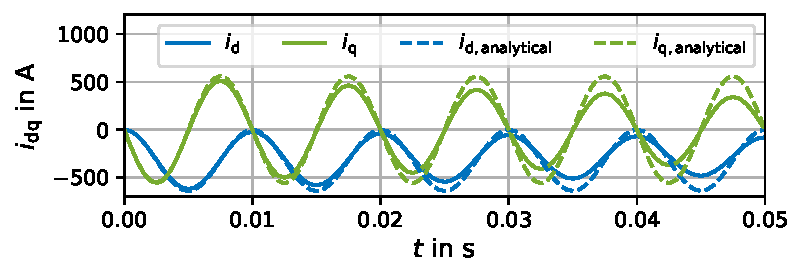
\includegraphics{ex06/i_dq_omega_const_analytical_ode.pdf}
        \caption{Transient process of $i_{\mathrm{dq}}$ of a salient synchronous machine with a stator and field winding short circuit.}
        \label{fig:i_dq_omega_const_analytical_ode}
    \end{solutionfigure}

    The trajectories of the field current $i_{\mathrm{f}}$ are visualized in \autoref{fig:i_f_omega_const_analytical_ode}. The behavior of this two trajectories are identical, except to the damping in the numerical solution, due to the considered winding resistance.
    \begin{solutionfigure}[ht]
        \centering
        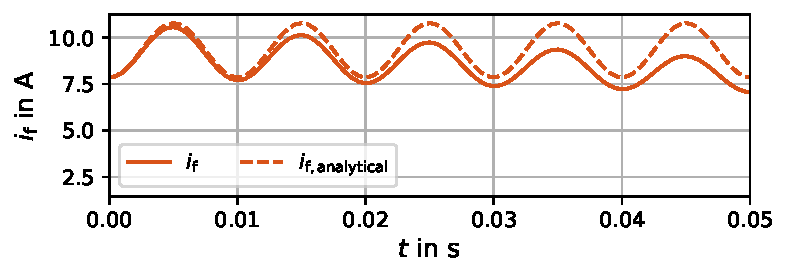
\includegraphics{ex06/i_f_omega_const_analytical_ode.pdf}
        \caption{Transient process of the field current $i_{\mathrm{f}}$ of a salient synchronous machine with a stator and field winding short circuit.}
        \label{fig:i_f_omega_const_analytical_ode}
    \end{solutionfigure}

\end{solutionblock}

\FloatBarrier

%%%%%%%%%%%%%%%%%%%%%%%%%%%%%%%%%%%%%%%%%%%%%%%%%%%%%%%%%%%%%
\subtask{Add a load with the following characteristic $T_{\mathrm{l}}(t) = 0.0001\cdot \omega_{\mathrm{r}}^{2}(t)$ to the existing simulation. Repeat the simulation with the same initial conditions as in the task before. Extend the simulation time to $T_{\mathrm{sim}} = \SI{0.5}{\second}$ and plot the currents $i_{\mathrm{d}}(t)$, $i_{\mathrm{f}}(t)$, the angular frequency of the rotor $\omega_{\mathrm{r,el}}(t)$ and the torque $T(t)$.}

\begin{solutionblock}
    The resulting currents for the new operating point are shown in \autoref{fig:i_dq_ode}.
    \begin{solutionfigure}[ht]
        \centering
        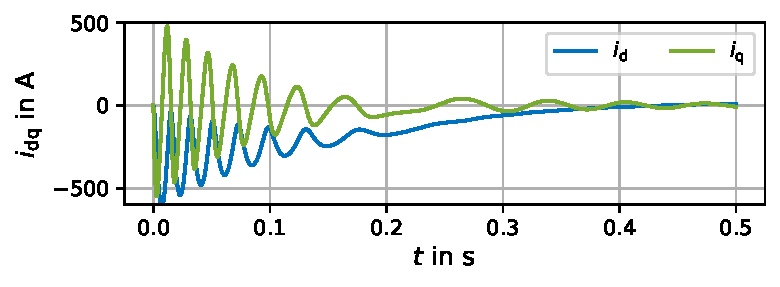
\includegraphics{ex06/i_dq_ode.pdf}
        \caption{Transient process of $i_{\mathrm{dq}}$ of a salient synchronous machine with a stator and field winding short circuit and a load resistance.}
        \label{fig:i_dq_ode}
    \end{solutionfigure}

    The filed winding current is visualized in \autoref{fig:i_f_ode}.
    \begin{solutionfigure}[ht]
        \centering
        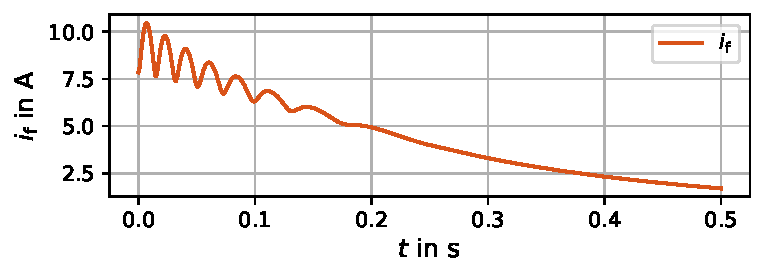
\includegraphics{ex06/i_f_ode.pdf}
        \caption{Transient process of $i_{\mathrm{f}}$ of a salient synchronous machine with a stator and field winding short circuit and a load resistance.}
        \label{fig:i_f_ode}
    \end{solutionfigure}

    Fig~\ref{fig:omega_r_el_ode} shows the angular frequency of the rotor. Due to the winding resistance and the additional load, the currents are reduced over time, until the machine comes to a standstill.
    \begin{solutionfigure}[ht]
        \centering
        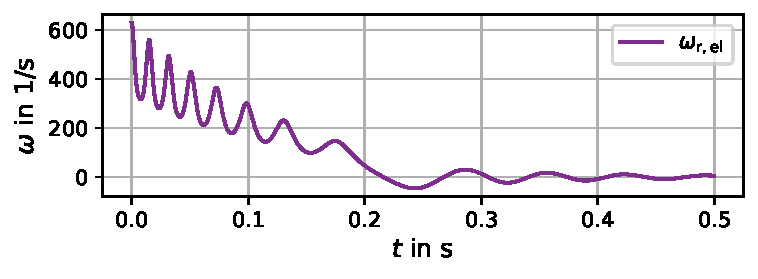
\includegraphics{ex06/omega_r_el_ode.pdf}
        \caption{Transient process of a salient synchronous machine with a stator and field winding short circuit and a load resistance.}
        \label{fig:omega_r_el_ode}
    \end{solutionfigure}

    The generated torque during the transient process is shown in \autoref{fig:T_ode}.
    \begin{solutionfigure}[ht]
        \centering
        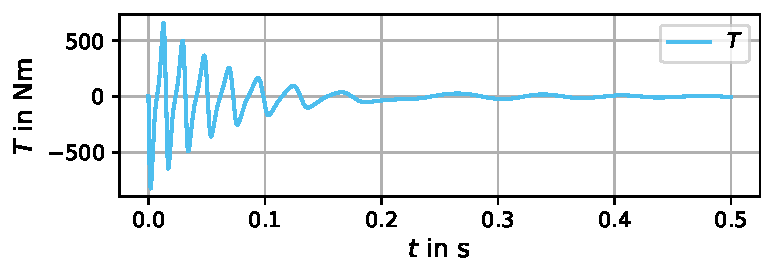
\includegraphics{ex06/T_ode.pdf}
        \caption{Generated torque of a salient synchronous machine with a stator and field winding short circuit and a load resistance.}
        \label{fig:T_ode}
    \end{solutionfigure}


\end{solutionblock}

\FloatBarrier

%%%%%%%%%%%%%%%%%%%%%%%%%%%%%%%%%%%%%%%%%%%%%%%%%%%%%%%%%%%%%
\subtask{Now consider an additional damper winding with the parameters from Tab.~\ref{tab:para_damperWinding} in the simulation. Compare the resulting current signalforms, the speed and the generated torque to the previous tasks with the identical simulation configuration as in the previous tasks. Consider the damper winding to not carry any current for $t$ = 0.}

\begin{table}[htb]
    \caption{Parameters of the damper winding.}
    \centering
    \begin{tabular}{lll}\toprule
    Symbol  & Description       & Value \\
    \midrule
    $M_{\mathrm{dD}}$   & Mutual ind. rotor d-axis  & $\SI{2}{\milli\henry}$ \\
    $M_{\mathrm{qQ}}$   & Mutual ind. rotor q-axis  & $\SI{1}{\milli\henry}$ \\
    $M_{\mathrm{fr}}$   & Mutual ind. field-rotor   & $\SI{50}{\milli\henry}$ \\
    $L_{\mathrm{D}}$    & Self ind. rotor d-axis    & $\SI{3}{\milli\henry}$ \\
    $L_{\mathrm{Q}}$    & Self ind. rotor q-axis    & $\SI{2}{\milli\henry}$ \\
    $R_{\mathrm{rD}}$   & Rotor winding res. d-axis & $\SI{50}{\milli\Omega}$ \\
    $R_{\mathrm{rQ}}$   & Rotor winding res. q-axis & $\SI{30}{\milli\Omega}$ \\
    \bottomrule
    \end{tabular}
    \label{tab:para_damperWinding}
\end{table}



\begin{solutionblock}
    With the additional damper winding, the stator flux linkage equation extends to
    \begin{equation}
        \begin{bmatrix}
            \psi_{\mathrm{s,d}}(t) \\
            \psi_{\mathrm{s,q}}(t)
        \end{bmatrix}
        =
        \begin{bmatrix}
            L_{\mathrm{s,d}}'   & 0 \\
            0   & L_{\mathrm{s,q}}'
        \end{bmatrix}
        \begin{bmatrix}
            i_{\mathrm{s,d}}(t) \\
            i_{\mathrm{s,q}}(t)
        \end{bmatrix}
        + M_{\mathrm{fs}}
        \begin{bmatrix}
            1 \\
            0
        \end{bmatrix}
        i_{\mathrm{f}}(t) +
        \begin{bmatrix}
            M_{\mathrm{dD}} & 0 \\
            0 & M_{\mathrm{qQ}}
        \end{bmatrix}
        \begin{bmatrix}
            i_{\mathrm{r,D}}(t) \\
            i_{\mathrm{r,Q}}(t)
        \end{bmatrix},
    \end{equation}

    and the field flux equation is extended with the rotor current as follows:
    \begin{equation}
        \psi_{\mathrm{f}}(t) = L_{\mathrm{f}}i_{\mathrm{f}}(t) + M_{\mathrm{f,s}}
        \begin{bmatrix}
            1 & 0
        \end{bmatrix}
        \begin{bmatrix}
            i_{\mathrm{s,d}}(t) \\
            i_{\mathrm{s,q}}(t)
        \end{bmatrix}
        + M_{\mathrm{fr}}
        \begin{bmatrix}
            1 & 0    
        \end{bmatrix}
        \begin{bmatrix}
            i_{\mathrm{r,D}}(t) \\
            i_{\mathrm{r,Q}}(t)
        \end{bmatrix}.
    \end{equation}

    The rotor flux equation is defined by:
    \begin{equation}
        \begin{bmatrix}
            \psi_{\mathrm{r,D}} \\
            \psi_{\mathrm{r,Q}}
        \end{bmatrix}
        =
        \begin{bmatrix}
            L_{\mathrm{s,d}} & 0 \\
            0   & L_{\mathrm{s,q}}
        \end{bmatrix}
        \begin{bmatrix}
            i_{\mathrm{r,D}}(t) \\
            i_{\mathrm{r,Q}}(t)
        \end{bmatrix}
        +
        \begin{bmatrix}
            M_{\mathrm{dD}}     & 0 \\
            0       & M_{\mathrm{qQ}}
        \end{bmatrix}
        \begin{bmatrix}
            i_{\mathrm{s,d}}(t) \\
            i_{\mathrm{s,q}}(t)
        \end{bmatrix}
        + M_{\mathrm{fr}}
        \begin{bmatrix}
            1 \\
            0
        \end{bmatrix}
        i_{\mathrm{f}}(t).
    \end{equation}


    In addition, also the torque equation changes to:
    \begin{equation}
        T(t) = \frac{3}{2}p\left[M_{\mathrm{fs}} i_{\mathrm{f}} i_{\mathrm{s,q}} + \left(L_{\mathrm{s,d}}' - L_{\mathrm{s,q}}'\right) i_{\mathrm{s,d}} i_{\mathrm{s,q}} + M_{\mathrm{dD}} i_{\mathrm{s,q}} i_{\mathrm{r,D}} - M_{\mathrm{qQ}} i_{\mathrm{s,d}} i_{\mathrm{r,Q}} \right].
    \end{equation}


    For the SM with damper winding, the flux linkage matrix extends to:
    \begin{equation}
        \bm{\psi} = 
        \begin{bmatrix}
            \psi_{\mathrm{s,d}}(t) \\
            \psi_{\mathrm{s,q}}(t) \\
            \psi_{\mathrm{f}}(t) \\
            \psi_{\mathrm{r,D}}(t) \\
            \psi_{\mathrm{r,Q}}(t)
        \end{bmatrix}
        =
        \underbrace{
        \begin{bmatrix}
            L_{\mathrm{s,d}}' & 0 & M_{\mathrm{fs}} & M_{\mathrm{dD}} & 0 \\
            0 & L_{\mathrm{s,q}}' & 0 & 0 & M_{\mathrm{qQ}} \\
            M_{\mathrm{fs}} & 0 & L_{\mathrm{f}} & M_{\mathrm{fr}} & 0 \\
            M_{\mathrm{dD}} & 0 & M_{\mathrm{fr}} & L_{\mathrm{D}} & 0 \\
            0 & M_{\mathrm{qQ}} & 0 & 0 & L_{\mathrm{Q}}
        \end{bmatrix}
        }_{\bm{L}}
        \begin{bmatrix}
            i_{\mathrm{s,d}}(t) \\
            i_{\mathrm{s,q}}(t) \\
            i_{\mathrm{f}}(t) \\
            i_{\mathrm{r,D}}(t) \\
            i_{\mathrm{r,Q}}(t)
        \end{bmatrix}.
    \end{equation}

    The differential current machine model with damping winding is defined as:
    \begin{equation}
        \frac{\mathrm{d}}{\mathrm{d}t}=
        \begin{bmatrix}
            i_{\mathrm{s,d}}(t) \\
            i_{\mathrm{s,q}}(t) \\
            i_{\mathrm{f}}(t) \\
            i_{\mathrm{r,D}}(t) \\
            i_{\mathrm{r,Q}}(t)
        \end{bmatrix}
        =
        \bm{L}^{-1}
        \begin{pmatrix}
            \begin{bmatrix}
                u_{\mathrm{s,d}}(t) \\
                u_{\mathrm{s,q}}(t) \\
                u_{\mathrm{f}}(t) \\
                u_{\mathrm{r,D}}(t) \\
                u_{\mathrm{r,Q}}(t)
            \end{bmatrix}
            -
            \begin{bmatrix}
                R_{\mathrm{s}} & 0 & 0 & 0 & 0 \\
                0 & R_{\mathrm{s}} & 0 & 0 & 0 \\
                0 & 0 & R_{\mathrm{f}} & 0 & 0 \\
                0 & 0 & 0 & R_{\mathrm{r,D}} & 0 \\
                0 & 0 & 0 & 0 & R_{\mathrm{r,Q}} \\
            \end{bmatrix}
            \begin{bmatrix}
                i_{\mathrm{s,d}}(t) \\
                i_{\mathrm{s,q}}(t) \\
                i_{\mathrm{f}}(t) \\
                i_{\mathrm{r,D}}(t) \\
                i_{\mathrm{r,Q}}(t)
            \end{bmatrix}
            -
            \begin{bmatrix}
                0 & -\omega_{\mathrm{r,el}}(t) & 0 & 0 & 0 \\
                \omega_{\mathrm{r,el}}(t) & 0 & 0  & 0 & 0 \\
                0 & 0 & 0 & 0 & 0 \\
                0 & 0 & 0 & 0 & 0 \\
                0 & 0 & 0 & 0 & 0 \\
            \end{bmatrix}
        \end{pmatrix}.
    \end{equation}

    In \autoref{fig:i_dq_dampingW_ode} the $i_{\mathrm{dq}}$ current trajectories during the transient process are shown.
    \begin{solutionfigure}[ht]
        \centering
        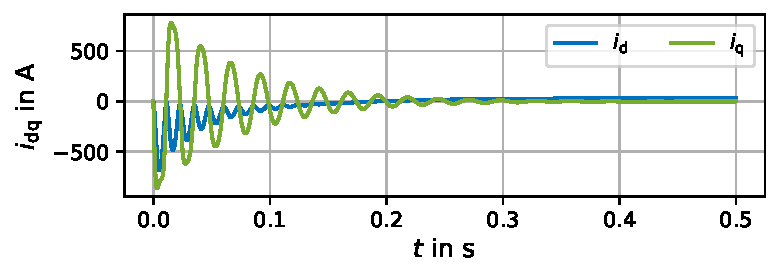
\includegraphics{ex06/i_dq_dampingW_ode.pdf}
        \caption{Transient process of a salient synchronous machine with a stator and field winding short circuit and a damper winding.}
        \label{fig:i_dq_dampingW_ode}
    \end{solutionfigure}

    The field current is visualized in \autoref{fig:i_f_dampingW_ode}.
    \begin{solutionfigure}[ht]
        \centering
        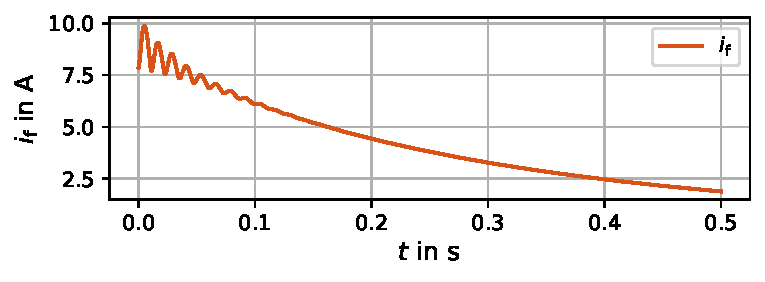
\includegraphics{ex06/i_f_dampingW_ode.pdf}
        \caption{Field current of a salient synchronous machine with a stator and field winding short circuit and a damper winding.}
        \label{fig:i_f_dampingW_ode}
    \end{solutionfigure}

    The rotational speed of the rotor is shown in \autoref{fig:omega_r_el_dampingW_ode}. The steady state is reached faster than in the simulation before, due to the added damping winding.
    \begin{solutionfigure}[ht]
        \centering
        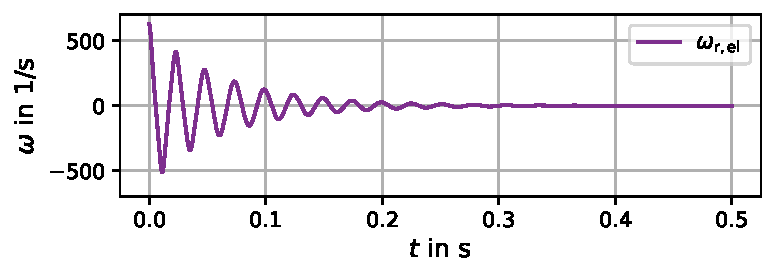
\includegraphics{ex06/omega_r_el_dampingW_ode.pdf}
        \caption{Speed of a salient synchronous machine with a stator and field winding short circuit and a damper winding.}
        \label{fig:omega_r_el_dampingW_ode}
    \end{solutionfigure}

    \autoref{fig:T_dampingW_ode} shows the generated torque during the transient process. The faster transient process is also visible in the torque curve, which faster converts to zero.
    \begin{solutionfigure}[ht]
        \centering
        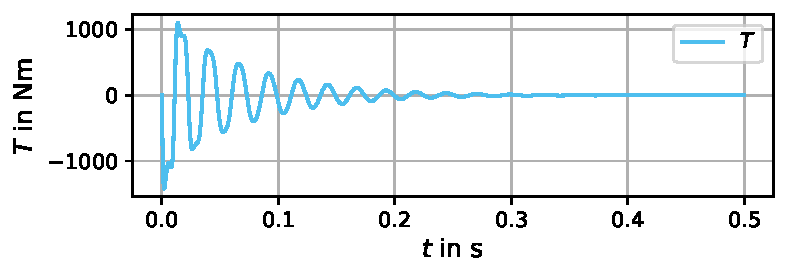
\includegraphics{ex06/T_dampingW_ode.pdf}
        \caption{Torque of a salient synchronous machine with a stator and field winding short circuit and a damper winding.}
        \label{fig:T_dampingW_ode}
    \end{solutionfigure}
\end{solutionblock}
\FloatBarrier

%%%%%%%%%%%%%%%%%%%%%%%%%%%%%%%%%%%%%%%%%%%%%%%%%%%%%%%%%%%%%
%% Task 2 %%
%%%%%%%%%%%%%%%%%%%%%%%%%%%%%%%%%%%%%%%%%%%%%%%%%%%%%%%%%%%%%

\task{Cylinderical synchronous machine}
In a thermal power station, a cylinderical synchronous generator is used which has the rated data in Tab.~\ref{tab:para_cylindericalSynchonousMachine} and is connected in star. The generator is driven by a turbine. The converted energy is fed into the 50 Hz national grid via a transformer. Saturation effects and losses in the machine can be neglected.
\begin{table}[htb]
    \caption{Parameters of the synchronous machine.}
    \centering
    \begin{tabular}{lll}\toprule
    Symbol  & Description       & Value \\
    \midrule
    $U_{\mathrm{star,n}}$ & Star voltage            & $\SI{\frac{10}{\sqrt{3}}}{\kilo\volt}$ \\
    $I_{\mathrm{star,n}}$ & Star current            & $\SI{6500}{\ampere}$ \\
    $f_{\mathrm{n}}$      & Nominal frequency       & $\SI{50}{\hertz}$ \\
    $\cos(\varphi_{\mathrm{n}})$    & Power factor  & 0.8 (capacitive) \\
    $n_{\mathrm{n}}$        & Nominal speed         & $\SI{1500}{\per\minute}$ \\
    $I_{\mathrm{f,n}}$    & Field current           & $\SI{150}{\ampere}$ \\ 
    $I_{\mathrm{s,sc0}}$  & Short circuit current   & $\SI{7800}{\ampere}$ \\
    \bottomrule
    \end{tabular}
    \label{tab:para_cylindericalSynchonousMachine}
\end{table}




%%%%%%%%%%%%%%%%%%%%%%%%%%%%%%%%%%%%%%%%%%%%%%%%%%%%%%%%%%%%%
\subtask{Synchronization must be carried out to connect the synchronous generator to the electricity grid. Why is this process necessary? Name the synchronization conditions that must be checked before the generator can be connected to the grid.}
\begin{solutionblock}
    Necessity of synchronization:
    \begin{itemize}
        \item Synchronization of the generator with the grid is absolutely essential for a complication-free connection of the machine to the grid. Otherwise, severe transient effects can lead to catastrophic effects.
        \item A high phase shift during the synchronization can start the machine to oscillate, but this is reduced by the damper winding in the rotor.
        \item In addition, connecting the generator with a large phase offset leads to high equalizing currents and thus a large torque are the result, which leads to the destruction of the generator.
    \end{itemize}

    Therefore, the following synchronization conditions should be fulfilled:
    \begin{itemize}
        \item The rotational frequency is equal to the grid frequency.
        \item The terminal voltage and the grid voltage are at the same level.
        \item The sense of rotation of the machine is equal to the grid.
        \item The phase orientation is equal to the grid.
    \end{itemize}

\end{solutionblock}




%%%%%%%%%%%%%%%%%%%%%%%%%%%%%%%%%%%%%%%%%%%%%%%%%%%%%%%%%%%%%
\subtask{How can the amount of active power output be influenced during generator operation? On the other hand, how can the inductive reactive power delivered or absorbed be influenced?}

\begin{solutionblock}
    The delivered active power can only be influenced by changing the mechanical input power. The delivered (over excitation) or absorbed (under excitation) reactive power is controlled via the field current.
\end{solutionblock}



%%%%%%%%%%%%%%%%%%%%%%%%%%%%%%%%%%%%%%%%%%%%%%%%%%%%%%%%%%%%%
\subtask{What is meant by synchronous condenser operation?}

\begin{solutionblock}
    In the synchronous condenser operation mode, only reactive power is delivered into or absorbed from the grid. The machine operates in no-load mode. This operation mode is used to control the reactive power within the grid. Sometimes, more or less reactive power is needed, dependant on the conditions of the considered time frame.
\end{solutionblock}

%%%%%%%%%%%%%%%%%%%%%%%%%%%%%%%%%%%%%%%%%%%%%%%%%%%%%%%%%%%%%
\subtask{Calculate with the given data the pole pair number $p$, the synchronous reactance $X_{\mathrm{s}}$, the apparent power $S$, the phase shift angle $\varphi$, the inner voltage $U_{\mathrm{i}}$ and the load angle $\theta$ at the rated conditions.}

\begin{solutionblock}
    The pole pair number is determined with:
    \begin{equation}
        p = \frac{\omega_{\mathrm{n}}}{\omega_{\mathrm{mech}}}
        = \frac{\SI{2\pi\cdot 50}{\per\second}}{\SI{2\pi \cdot 25}{\per\second}}
        = 2.
    \end{equation}

    The synchronous reactance is calculated by
    \begin{equation}
        X_{\mathrm{s}} = \frac{U_{\mathrm{s}}}{I_{\mathrm{s,sc0}}}
        = \frac{\SI{\frac{10000}{\sqrt{3}}}{\volt}}{\SI{7800}{\ampere}}
        = \SI{0.74}{\Omega},
    \end{equation}
    with the stator voltage $U_{\mathrm{s}}$ and the short circuit current $I_{\mathrm{s,sc0}}$.
    The apparent power determines as
    \begin{equation}
        S = \sqrt{3} U_{\mathrm{n}} I_{\mathrm{n}}
        = \sqrt{3}\cdot \SI{10000}{\volt}\cdot\SI{6500}{\ampere}
        = \SI{112.58}{\mega\volt\ampere},
    \end{equation}
    and this leads to the calculation of the phase shift angle by:
    \begin{equation}
        \varphi = \arccos(-0.8)\cdot \mathrm{sign}\left(\frac{Q}{S}\right)
        = - \arccos(-0.8) = \SI{-143.13}{\degree}.
    \end{equation}

    The inner voltage is calculated with
    \begin{equation}
        U_{\mathrm{i}} = X_{\mathrm{s}} I_{\mathrm{s,sc}}
        = X_{\mathrm{s}} \left(\frac{I_{\mathrm{s,sc0}}-I_{\mathrm{s}}\sin(\varphi)}{\cos(\varphi)}\right),
    \end{equation}
    and the active power is defined as:
    \begin{equation}
        P = \frac{3 U_{\mathrm{s}}U_{\mathrm{i}}}{X_{\mathrm{s}}} \sin(\theta).
    \end{equation}
    Inserting the inner voltage from above into the active power equation, yields:
    \begin{equation}
        P = \frac{3 U_{\mathrm{s}} X_{\mathrm{s}} \left(\frac{I_{\mathrm{s,sc0}}-I_{\mathrm{s}}\sin(\varphi)}{\cos(\varphi)}\right)}{X_{\mathrm{s}}} \sin(\theta)
        = 3 U_{\mathrm{s}} \left(I_{\mathrm{s,sc0}}-I_{\mathrm{s}} \sin(\varphi)\right) \tan(\theta).
    \end{equation}

    Hence, the load angle is determined with resorting the equation from above as follows:
    \begin{align}
        \begin{split}
        \theta &= \arctan\left(\frac{P}{3 U_{\mathrm{s}}(I_{\mathrm{s,sc0}}-I_{\mathrm{s,sc}}\sin(\varphi))}\right)
        =\arctan\left(\frac{3 U_{\mathrm{s}} I_{\mathrm{s}} \cos(\varphi)}{3 U_{\mathrm{s}}(I_{\mathrm{s,sc0}}-I_{\mathrm{s,sc}}\sin(\varphi))}\right) \\
        &= \arctan\left(\frac{I_{\mathrm{s}}\cos(\varphi)}{I_{\mathrm{s,sc0}}-I_{\mathrm{s}}\sin(\varphi)} \right)
        = \arctan\left(\frac{\SI{6.5}{\kilo\ampere}\cdot \cos(\SI{-143.13}{\degree})}{\SI{7.8}{\kilo\ampere}-\SI{6.5}{\kilo\ampere}\cdot\sin(\SI{-143.13}{\degree})}\right)
        = \SI{-23.95}{\degree}.
        \end{split}
        \label{eq:load_angle}
    \end{align}

    The inner voltage is calculated by:
    \begin{equation}
        U_{\mathrm{i}} = X_{\mathrm{s}} I_{\mathrm{s,sc}}
        = X_{\mathrm{s}} \left(\frac{I_{\mathrm{s,sc0}}- I_{\mathrm{s}}\sin(\varphi)}{\cos(\theta)}\right)
        = \SI{0.74}{\Omega}\cdot\left(\frac{\SI{7.8}{\kilo\ampere}-\SI{6.5}{\kilo\ampere}\cdot\sin(\SI{-143.13}{\degree})}{\cos(\SI{-23.95}{\degree})}\right)
        = \SI{9473}{\volt}.
    \end{equation}
\end{solutionblock}


%%%%%%%%%%%%%%%%%%%%%%%%%%%%%%%%%%%%%%%%%%%%%%%%%%%%%%%%%%%%%
\subtask{The generator should only take reactive power from the grid. How large is the stator current $I_{\mathrm{s}}$ and the field current $I_{\mathrm{f}}$ at this operating point, when a reactive power of 120 MVA is extracted from the grid? How large is the phase shift angle $\varphi$ and the load angle $\theta$? Draw the phasor diagram for this operating point.}

\begin{solutionblock}
    The stator current changes to
    \begin{equation}
        I_{\mathrm{s}} = \frac{Q}{\sqrt{3}U_{\mathrm{n}}\sin(\varphi)}
        = \frac{\SI{120}{\mega\volt\ampere}}{\SI{\sqrt{3}\cdot10}{\kilo\volt}}
        = \SI{6928.2}{\ampere},
    \end{equation}

    and the inner voltage is determined with:
    \begin{equation}
        U_{\mathrm{i}} = \frac{3 U_{\mathrm{s}}^2 - X_{\mathrm{s}}Q}{3U_{\mathrm{s}}\cos(\theta)}
        = \frac{3\cdot\left(\frac{\SI{10}{\kilo\volt}}{\sqrt{3}}\right)^2 - \SI{0.74}{\Omega}\cdot\SI{120}{\mega\volt\ampere}}{3\cdot\frac{\SI{10}{\kilo\volt}}{\sqrt{3}}\cos(\SI{0}{\degree})}
        = \SI{1501.11}{\volt}.
    \end{equation}

    Therefore, the necessary field current results in
    \begin{equation}
        I_{\mathrm{f}} = \frac{U_{\mathrm{i}}}{U_{\mathrm{i,n}}}I_{\mathrm{f,n}}
        = \frac{\SI{1501.11}{\volt}}{\SI{9473}{\volt}}\cdot \SI{150}{\ampere}
        = \SI{23.77}{\ampere}.
    \end{equation}

    The phase shift angle is $\varphi = \SI{90}{\degree}$ and the load angle is $\theta = \SI{0}{\degree}$. The phasor diagram is visualized in \autoref{fig:Phasor_diagram_reactive}, the inner voltage $\underline{U}_{\mathrm{i}}$ is purely imaginary, as defined in the lecture notes. The stator voltage $\underline{U}_{\mathrm{s}}$ and the internal voltage are directly on top of each other due to the zero load angle $\theta$.
    \begin{solutionfigure}[ht]
        \centering
        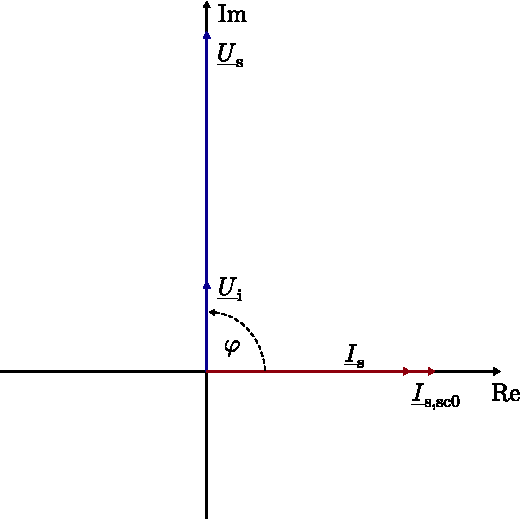
\includegraphics{ex06/Phasor_diagram_reactive.pdf}
        \caption{Phasor diagram for the given operating point. The scala is for the voltage 1 cm $\widehat{=}~ \SI{1000}{\volt}$ and for the current 1 cm $\widehat{=}~ \SI{2000}{\ampere}$.}
        \label{fig:Phasor_diagram_reactive}
    \end{solutionfigure}

\end{solutionblock}


%%%%%%%%%%%%%%%%%%%%%%%%%%%%%%%%%%%%%%%%%%%%%%%%%%%%%%%%%%%%%
\subtask{In contrast to the previous subtask, the generator should provide 80 MW in addition to the reactive power now. How large is the stator current $I_{\mathrm{s}}$, the phase shift angle $\varphi$ and the load angle $\theta$? Draw also for this operation point the phasor diagram.}

\begin{solutionblock}
    
    The apparent power is:
    \begin{equation}
        S = \sqrt{P^2+Q^2}
        = \sqrt{\left(\SI{80}{\mega\watt}\right)^2 + \left(\SI{120}{\mega\volt\ampere}\right)^2}
        = \SI{144.22}{\mega\volt\ampere}.
    \end{equation}

    Hence, the stator current yields:
    \begin{equation}
        I_{\mathrm{s}} = \frac{S}{\sqrt{3}U_{\mathrm{n}}}
        = \frac{\SI{144.22}{\mega\volt\ampere}}{\sqrt{3}\cdot\SI{10}{\kilo\volt}}
        = \SI{8326.54}{\ampere}.
    \end{equation}

    Retrieving the power factor via the complex power equation leads to:
    \begin{equation}
        \varphi = \arccos\left(\frac{-P}{\sqrt{3}U_{\mathrm{s,n}}I_{\mathrm{s}}} \right)
        = \arccos\left(\frac{-\SI{80}{\mega\watt}}{\sqrt{3}\cdot\SI{10}{\kilo\volt}\cdot\SI{8326.54}{\ampere}}\right)
        = \SI{123.7}{\degree}.
    \end{equation}

    The derivation of the load angle is already given in \eqref{eq:load_angle}, which results for the new operation point in
    \begin{equation}
        \theta = \arctan\left(\frac{I_{\mathrm{s}}\cos(\varphi)}{I_{\mathrm{s,sc0}}-I_{\mathrm{s}}\sin(\varphi)}\right)
        = \SI{-79.66}{\degree},
    \end{equation}
    while the resulting inner voltage is
    \begin{equation}
        U_{\mathrm{i}} = X_{\mathrm{s}} I_{\mathrm{s,sc}}
        = \SI{3600}{\volt}.
    \end{equation}

    The phasor diagram is visualized in \autoref{fig:Phasor_diagram_reactive_active}, the inner voltage $\underline{U}_{\mathrm{i}}$ is purely imaginary, as defined in the lecture notes.
    \begin{solutionfigure}
        \centering
        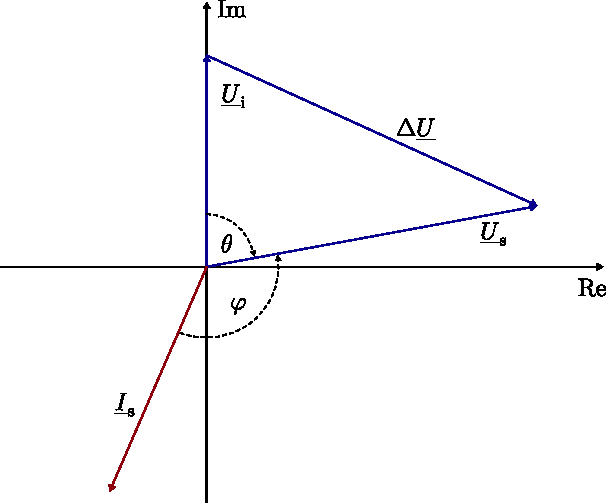
\includegraphics{ex06/Phasor_diagram_reactive_active.pdf}
        \caption{Phasor diagram for the given operating point. The scala is for the voltage 1 cm $\widehat{=}~ \SI{1000}{\volt}$ and for the current 1 cm $\widehat{=}~ \SI{2000}{\ampere}$.}
        \label{fig:Phasor_diagram_reactive_active}
    \end{solutionfigure}


\end{solutionblock}



%%%%%%%%%%%%%%%%%%%%%%%%%%%%%%%%%%%%%%%%%%%%%%%%%%%%%%%%%%%%%
\subtask{Now, the generator should provide a reactive power of 60 MVA into the grid. How large is the generated torque $T$, that the generator operates within the rated apparent power? To which value must the field current $I_{\mathrm{f}}$ change, such that the rated current is reached in the stator winding?}

\begin{solutionblock}
    With the determined rated apparent power in the task before, the given reactive power, the maximum power is calculated by
    \begin{equation}
        P = \sqrt{S_{\mathrm{n}}^2 - Q^2}
        = \sqrt{\left(\SI{112.58}{\mega\volt\ampere}\right)^2 - \left(\SI{60}{\mega\volt\ampere}\right)^2}
        = \SI{95.26}{\mega\watt},
    \end{equation}
    hence, the maximum torque is given with:
    \begin{equation}
        T_{\mathrm{max}} = \frac{P}{\omega_{\mathrm{mech,n}}}
        = \frac{\SI{95.26}{\mega\watt}}{\SI{2\pi\cdot 25}{\per\second}}
        = \SI{606.5}{\kilo\newton\metre}.
    \end{equation}
    

    The angle $\varphi$ for the phase shift at nominal current is determined as:
    \begin{equation}
        \varphi = \arccos\left(\frac{P}{\sqrt{3}U_{\mathrm{star,n} I_{\mathrm{star,n}}}}\right)
        = \arccos\left(\frac{-\SI{95.26}{\mega\watt}}{\sqrt{3}\cdot \SI{10}{\kilo\volt}\cdot \SI{6.5}{\kilo\ampere}}\right)
        = -\SI{147.8}{\degree}.
    \end{equation}

    With \eqref{eq:load_angle} the load angle is calculated by
    \begin{equation}
        \theta = \arccos\left(\frac{I_{\mathrm{s}}\cos(\varphi)}{I_{\mathrm{s,sc0}}-I_{\mathrm{s,sc}}\sin(\varphi)}\right)
        = \arctan\left(\frac{\SI{6.5}{\kilo\ampere}\cos(\SI{-147.8}{\degree})}{\SI{7.8}{\kilo\ampere}-\SI{6.5}{\kilo\ampere}\sin(\SI{-147.8}{\degree})}\right)
        = \SI{-26.03}{\degree},
    \end{equation}
    therefore, the inner voltage results into:
    \begin{equation}
        U_{\mathrm{i}} = X_{\mathrm{s}} I_{\mathrm{s,sc}}
        = X_{\mathrm{s}} \left(\frac{I_{\mathrm{s,sc0}}-I_{\mathrm{s}}\sin(\varphi)}{\cos(\theta)}\right)
        = \SI{0.74}{\Omega}\left(\frac{\SI{7.8}{\kilo\ampere}-\SI{6.5}{\kilo\ampere}\sin(\SI{-147.8}{\degree})}{\cos(\SI{-26.03}{\degree})}\right)
        = \SI{9276}{\volt}.
    \end{equation}

    The field current must be set to the following value:
    \begin{equation}
        I_{\mathrm{f}} = \frac{U_{\mathrm{i}}}{U_{\mathrm{i,n}}}I_{\mathrm{f,n}}
        = \frac{\SI{9276}{\volt}}{\SI{9473}{\volt}}\cdot \SI{150}{\ampere}
        = \SI{146.9}{\ampere}.
    \end{equation}

\end{solutionblock}

\FloatBarrier


%%%%%%%%%%%%%%%%%%%%%%%%%%%%%%%%%%%%%%%%%%%%%%%%%%%%%%%%%%%%%
%% Task 3 %%
%%%%%%%%%%%%%%%%%%%%%%%%%%%%%%%%%%%%%%%%%%%%%%%%%%%%%%%%%%%%%

\task{Steady-state operation of a synchronous machine}
Consider a loss-free synchronous machine with the parameters from Tab.~\ref{tab:para_SynchonousMachine}. First, the synchronous machine is operated as a a motor. Using the data given above, determine the following characteristic variables of the synchronous machine at rated operation. An example phasor diagram for this operation is shown in \autoref{fig:Phasor_diagrams_m_oe}.


\begin{table}[htb]
    \caption{Parameters of the synchronous machine.}
    \centering
    \begin{tabular}{lll}\toprule
    Symbol  & Description       & Value \\
    \midrule
    $U_{\mathrm{star,n}}$ & Star voltage            & $\SI{\frac{6}{\sqrt{3}}}{\kilo\volt}$ \\
    $I_{\mathrm{star,n}}$ & Star current            & $\SI{96}{\ampere}$ \\
    $f_{\mathrm{n}}$      & Nominal frequency       & $\SI{50}{\hertz}$ \\
    $p$                   & Pole pair number        & 2 \\
    $\cos(\varphi_{\mathrm{n}})$    & Power factor  & 0.9 (capacitive) \\
    $T_{\mathrm{n}}$      & Nominal torque          & $\frac{T_{\mathrm{max}}}{2}$ \\
    \bottomrule
    \end{tabular}
    \label{tab:para_SynchonousMachine}
\end{table}

\begin{figure}[ht]
    \centering
    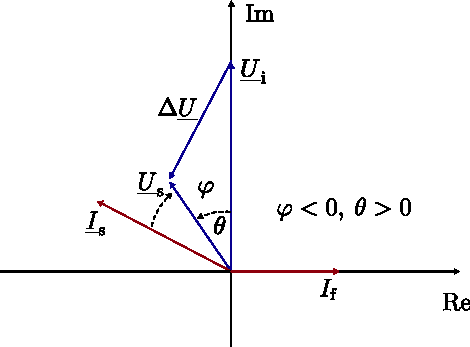
\includegraphics{ex06/Phasor_diagrams_m_oe.pdf}
    \caption{Phasor diagram of a over excited synchronous machine in motor mode.}
    \label{fig:Phasor_diagrams_m_oe}
\end{figure}

%%%%%%%%%%%%%%%%%%%%%%%%%%%%%%%%%%%%%%%%%%%%%%%%%%%%%%%%%%%%%
\subtask{How large is the maximum torque $T_{\mathrm{max}}$?}

\begin{solutionblock}

    Due to the ideal machine characteristic (no losses), the nominal torque is calculated by
    \begin{equation}
        T_{\mathrm{n}} = \frac{P_{\mathrm{n}}}{\omega_{\mathrm{mech,n}}}
        = \frac{3 U_{\mathrm{star,n}} I_{\mathrm{star,n}} \cos(\varphi)}{\omega_{\mathrm{mech,n}}}
        = \frac{\sqrt{3}\cdot \SI{6000}{\volt}\cdot\SI{96}{\ampere}\cdot0.9}{\SI{2\pi\cdot50}{\per\second}}
        = \SI{2858}{\newton\metre},
    \end{equation}

    and, the maximum torque calculates as follows:
    \begin{equation}
        T_{\mathrm{max}} = 2 T_{\mathrm{n}}
        = 2 \cdot \SI{2858}{\newton\metre}
        = \SI{5716}{\newton\metre}.
    \end{equation}
    
\end{solutionblock}



%%%%%%%%%%%%%%%%%%%%%%%%%%%%%%%%%%%%%%%%%%%%%%%%%%%%%%%%%%%%%
\subtask{Which load angle $\theta$ is set at the nominal operating point?}

\begin{solutionblock}
    The load angle can be determined by geometric transformations, which are shown in \autoref{fig:syn_motor_overExcited}.
    \begin{solutionfigure}
        \centering
        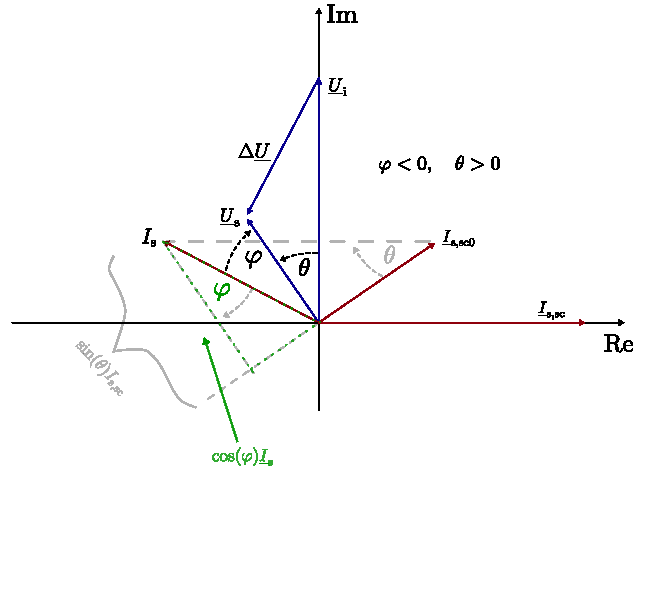
\includegraphics{ex06/syn_motor_overExcited.pdf}
        \caption{Phasor diagram for an over excited synchronous machine in motor operation.}
        \label{fig:syn_motor_overExcited}
    \end{solutionfigure}
    
    The target is to create two different triangles, one with the known angle $\varphi$ (marked in green in the figure) and one without the load angle $\theta$ (marked in gray in the figure). 
    Hence, the load angle calculates as follows
    \begin{align}
        \begin{split}
            \sin(\theta) I_{\mathrm{s,sc}} = \cos(\varphi)I_{\mathrm{s}},\\
            \sin(\theta) = \frac{I_{\mathrm{s}}}{I_{\mathrm{s,sc}}}\cos(\varphi),
        \end{split}
    \end{align}
    which leads to the angle:
    \begin{equation}
        \theta = \arcsin\left(\frac{I_{\mathrm{s}}}{I_{\mathrm{s,sc}}} \right) \cos(\varphi)
        = \arcsin\left(\frac{\SI{96}{\ampere}}{\SI{172.8}{\ampere}}\right) \cdot 0.9
        = \SI{30}{\degree}.
    \end{equation}
\end{solutionblock}

%%%%%%%%%%%%%%%%%%%%%%%%%%%%%%%%%%%%%%%%%%%%%%%%%%%%%%%%%%%%%
\subtask{Determine the synchronous reactance $X_{\mathrm{s}}$ value.}

\begin{solutionblock}
    The reactance is determined as:
    \begin{align}
        \begin{split}
        X_{\mathrm{s}}
        &= \frac{U_{\mathrm{i}}}{I_{\mathrm{s,sc}}}
        = \frac{U_{\mathrm{s}}}{I_{\mathrm{s,sc0}}}
        = \frac{U_{\mathrm{s}}}{I_{\mathrm{s}}\sin(\arccos(0.9)\mathrm{sign}(Q/S))+I_{\mathrm{s,sc}}\cos(\theta)} \\
        &= \frac{\SI{\frac{6000}{\sqrt{3}}}{\volt}}{\SI{96}{\ampere}\cdot \sin(\SI{-25.8}{\degree}) + \SI{172.8}{\ampere}\cdot \cos(\SI{30}{\degree})}
        = \SI{32.12}{\Omega}.
        \end{split}
    \end{align}

\end{solutionblock}


%%%%%%%%%%%%%%%%%%%%%%%%%%%%%%%%%%%%%%%%%%%%%%%%%%%%%%%%%%%%%
\subtask{Calculate the inner voltage $U_{\mathrm{i}}$ at the nominal operating point.}
\begin{solutionblock}
    
    \begin{equation}
        U_{\mathrm{i}} = X_{\mathrm{s}} I_{\mathrm{s,sc}}
        = \SI{32.12}{\Omega} \cdot \SI{172.79}{\ampere}
        = \SI{5549.52}{\volt}
    \end{equation}
\end{solutionblock}




%%%%%%%%%%%%%%%%%%%%%%%%%%%%%%%%%%%%%%%%%%%%%%%%%%%%%%%%%%%%%
\subtask{In the next task, the machine operates as generator and the power is 500 kW. The phasor diagram for this operation is shown in \autoref{fig:Phasor_diagrams_gen_oe}. Which load angle $\theta$ is set at the new operating point?}

\begin{figure}[ht]
    \centering
    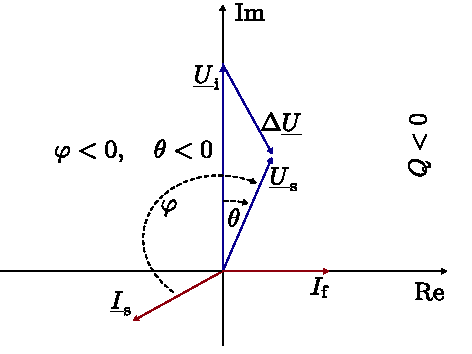
\includegraphics{ex06/Phasor_diagrams_gen_oe.pdf}
    \caption{Phasor diagram of an over excited synchronous machine in generator mode.}
    \label{fig:Phasor_diagrams_gen_oe}
\end{figure}


\begin{solutionblock}
    In the generator mode, the load angle is negative. With the generated power of 500 kW and the constant voltage, the product of the current and power factor is determined by:
    \begin{equation}
        \cos(\varphi) I_{\mathrm{s}} = \frac{P}{3 U_{\mathrm{s}}}
        = \frac{\SI{-500}{\kilo\watt}}{3\cdot \SI{\frac{6000}{\sqrt{3}}}{\volt}}
        = -\SI{48.11}{\ampere}.
    \end{equation}

    It is also assumed that the short-circuit current has not changed its value by maintaining the excitation current. The load angle can now be determined using the trigonometric relationship:
    \begin{equation}
        \theta = \arcsin\left(\frac{I_{\mathrm{s}}}{I_{\mathrm{s,sc}}}\cos(\varphi)\right)
        = \arcsin\left(\frac{\SI{-48.11}{\ampere}}{\SI{172.8}{\ampere}}\right)
        = \SI{-16.17}{\degree}.
    \end{equation}
\end{solutionblock}


%%%%%%%%%%%%%%%%%%%%%%%%%%%%%%%%%%%%%%%%%%%%%%%%%%%%%%%%%%%%%
\subtask{Calculate the stator current $I_{\mathrm{s}}$.}

\begin{solutionblock}
    The stator current is calculated with the active and the reactive current components, which are defined as in the previous task by
    \begin{equation}
        I_{\mathrm{s}} = \sqrt{I_{\mathrm{active}}^2 + I_{\mathrm{reactive}}^2}
        = \sqrt{\left(I_{\mathrm{s}}\sin(-\varphi - \SI{90}{\degree})\right)^2 + \left(I_{\mathrm{s}}\cos(-\varphi - \SI{90}{\degree})\right)^2}.
    \end{equation}
    
    With the relationship between the trigonometric functions and the phase shift, the equation from above is resorted to:
    \begin{align}
        \begin{split}
            I_{\mathrm{s}} &= \sqrt{\left(-I_{\mathrm{s}}\cos(-\varphi)\right)^2 + \left(I_{\mathrm{s}}\sin(-\varphi)\right)^2} \\
            & = \sqrt{\left(-I_{\mathrm{s}}\cos(-\varphi)\right)^2 + \left(-I_{\mathrm{s}}\sin(\varphi)\right)^2}.
        \end{split}
    \end{align}

    With the triangular relationship:
    \begin{align}
        \begin{split}
        I_{\mathrm{s}} &= \sqrt{\left(-I_{\mathrm{s}}\cos(-\varphi)\right)^2 + \left(I_{\mathrm{s,sc0}}-I_{\mathrm{s,sc}}\cos(\theta)\right)^2} \\
        &= \sqrt{\left(-I_{\mathrm{s}}\cos(-\varphi)\right)^2 + \left(I_{\mathrm{s,sc0}}+I_{\mathrm{s,sc}}\cos(\theta)\right)^2}.
        \end{split}
    \end{align}

    Use the calculation of the short circuit current $I_{\mathrm{s,sc0}}$, leads to:
    \begin{align}
        \begin{split}
            I_{\mathrm{s}} &= \sqrt{\left(-I_{\mathrm{s}}\cos(-\varphi)\right)^2 + \left(-\frac{U_{\mathrm{s}}}{X_{\mathrm{s}}}+I_{\mathrm{s,sc}}\cos(\theta)\right)^2} \\
            &= \sqrt{\left(\SI{48.11}{\ampere}\right)^2 + \left(-\frac{\SI{\frac{6000}{\sqrt{3}}}{\volt}}{\SI{32.12}{\Omega}} + \SI{172.79}{\ampere}\cos(-\SI{16.17}{\degree})\right)^2} \\
            &= \SI{75.44}{\ampere}.
        \end{split}
    \end{align}

\end{solutionblock}


%%%%%%%%%%%%%%%%%%%%%%%%%%%%%%%%%%%%%%%%%%%%%%%%%%%%%%%%%%%%%
\subtask{How large is the power factor $\cos(\varphi)$ at this operating point? In addition, calculate the angle $\varphi$.}

\begin{solutionblock}
    The active power is calculated with
    \begin{equation}
        I_{\mathrm{active}} = I_{\mathrm{s}} \cos(\varphi),
    \end{equation}
    which than leads to
    \begin{equation}
        \cos(\varphi) = \frac{I_{\mathrm{active}}}{I_{\mathrm{s}}} 
        = \frac{I_{\mathrm{s}}\cos(\varphi)}{I_{\mathrm{s}}}
        = \frac{-\SI{48.11}{\ampere}}{\SI{75.44}{\ampere}}
        = -0.638,
    \end{equation}
    and, therefore, the angle results into:
    \begin{equation}
        \varphi = \arccos(-0.638)\cdot \mathrm{sign}\left(\frac{Q}{S}\right)
        = -\arccos(-0.638) = \SI{-129.6}{\degree}.
    \end{equation}
\end{solutionblock}








